\chapter*{Introduction}
\phantomsection
\addstarredchapter{\textbf{Introduction}}

\fancyhead[LE]{\thepage} 
\fancyhead[RE]{\textbf{Introduction}}
\fancyhead[RO]{\thepage} 
\fancyhead[LO]{\textbf{Introduction}}
\fancyfoot[C]{\thepage}

\setlength{\parindent}{0.35cm} 

% ====================================================

The visualization tool \cwv~was developed with the aim of visualizing the modelling outputs of the \cws\cwversion~modelling platform. This extension currently operates as a QGIS plugin under QGIS version \qgisversion and the same functionalities are as well accessible via API through jupyter notebook \label{sec-notebook-usage}.\\

\cwv~is structured around various tools and features that assist in the calibration process of a \cawaqs~application and facilitate the visualization of time series and the spatial distribution of simulated hydrological variables.

\cwv~is built on top of a standalone scientific backend HTAS \href{https://github.com/flipoyo/HydrologicalTwinAlphaSeries}{(HydrologicalTwinAlphaSeries)} and consumes it through a well-defined public interface. 

\Cref{fig-cvz-ecosystem} situates the plug-in within the wider \cawaqs~toolchain.
\begin{figure}[H]
    \centering
    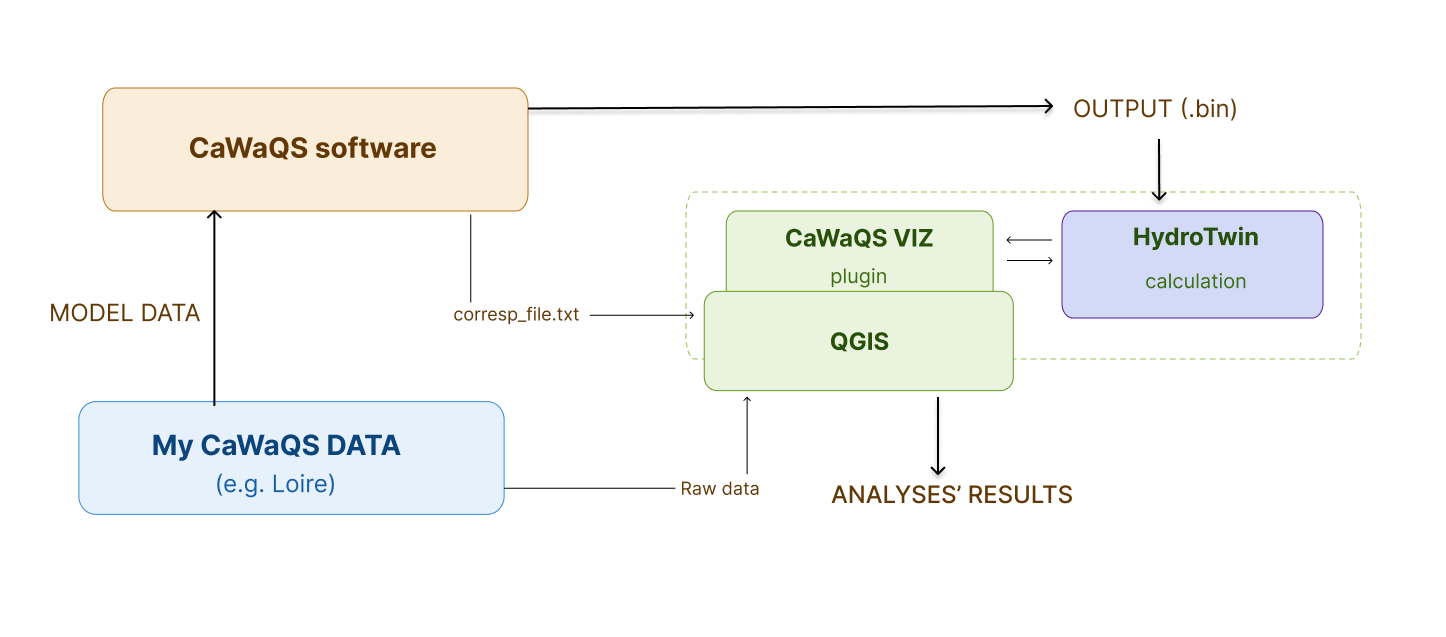
\includegraphics[width=0.9\linewidth]{4_application_scripts/fig/cvz_ecosystem.png}
    \caption{The \cwv~ecosystem --- position of the plug-in within the \cawaqs~toolchain.}
    \label{fig-cvz-ecosystem}
\end{figure}